\documentclass[12pt,letterpaper,noanswers]{exam}
\usepackage[usenames,dvipsnames,svgnames,table]{xcolor}
\usepackage[margin=0.9in]{geometry}
\renewcommand{\familydefault}{\sfdefault}
\usepackage{multicol}
\pagestyle{head}
\definecolor{c03}{HTML}{FFDDDD}
\header{AM 108 Class 13}{}{Poincar\'e Index}
\runningheadrule
\headrule
\usepackage{graphicx} % more modern
\usepackage{amsmath} 
\usepackage{amssymb} 
\usepackage{hyperref}
\usepackage{tcolorbox}

\begin{document}
 \pdfpageheight 11in 
  \pdfpagewidth 8.5in

\noindent 




\begin{itemize}
    \item There is a problem set due Friday October 9th.
    \item There is a pre-class assignment for Wednesday.
    \item There is a skill check in class on Wednesday.  The problem info is below.
\end{itemize}

\hrule
\vspace{0.2cm}





\noindent\textbf{Teams}

\begin{multicols}{2}
1. 

\end{multicols}

\noindent \textbf{Teams 3 and 4}: Post screenshots of your work to the course Google Drive today.  Include words, labels, and other short notes that might make those solutions useful to you or your classmates.  Find the link in Canvas (or here: \url{https://drive.google.com/drive/u/0/folders/1GcpwvKHD4tMecpFQ4lNxN_r5Ylj7YHbd})

\vspace{0.2cm}

\hrule
\vspace{0.2cm}

\noindent\textbf{Big picture}

We have been learning methods for constructing a phase portrait for a 2d system (a much bigger undertaking that constructing phase portraits on the line in 1d).  The Poincar\'e index provides our first non-local information about the phase portrait.  We can use it to identify possible locations of closed trajectories in a 2d system.

Next, we will learn methods for ruling out closed trajectories and one method that allows us to show a closed trajectory exists.

\vspace{0.2cm}

\hrule
\vspace{0.2cm}

\noindent \textbf{Extra vocabulary / extra facts:}
\begin{tcolorbox}
A \textbf{Jordan curve} $C$ is a piecewise-smooth, simple (doesn't cross itself), closed curve.

The \textbf{index} (sometimes \textbf{Poincar\'e index}) of a Jordan curve $C$ relative to a vector field $\underline{f}$ that is continuous in $\mathbb{R}^2$, where $\underline f$ doesn't have a critical point on the curve $C$, is defined as the integer $I_{\underline f}(C) = \frac{\Delta \Theta}{2\pi}$, where $\Delta\Theta$ is the total change in the angle $\Theta$ that the vector $\underline f$ makes with respect to the $x$-axis traversing $C$ exactly once in the positive (counterclockwise) direction. (Definition taken from Perko 1996.)

A vector $\left(\begin{array}{c} f(x,y) \\ g(x,y) \end{array}\right)$ makes the angle $\Theta(x,y) = \tan^{-1} \frac{g(x,y)}{f(x,y)}$ with the $x$-axis.
\end{tcolorbox}
\begin{tcolorbox}
We can compute $\Delta\Theta$ via a line integral (path integral).  Specifically, $\displaystyle \Delta\Theta = \oint_C d\Theta = \oint_C d\tan^{-1}\frac{g(x,y)}{f(x,y)}$.  Note that $\frac{d}{dx}\tan^{-1} x = \frac{1}{1+x^2}$.  Using the chain rule to compute the differential $d\tan^{-1}\frac{g}{f}$, we have $d\tan^{-1}\frac{g}{f} = \frac{1}{1+(g/f)^2}\left(dg/f -gdf/f^2\right)$, so $\displaystyle d\tan^{-1}(g/f) = (dg/f - gdf/f^2)f^2/(f^2+g^2)= \frac{fdg - gdf}{f^2+g^2}$, where $df = f_x dx + f_ydy$ and $dg = g_xdx + g_ydy$.  Reorganizing, the line integral becomes $\displaystyle\oint_C d\Theta = \oint_C \frac{1}{f^2+g^2}\left((fg_x-gf_x)dx+(fg_y-gf_y)dy\right) = \oint_C \frac{1}{f^2+g^2}((fg_x-gf_x)\vec i +(fg_y-gf_y)\vec j)\cdot d\underline r$

\end{tcolorbox}



\vspace{0.2cm}
\hrule
\vspace{0.2cm}

\noindent\textbf{Your questions}
\begin{enumerate}
    \item Is a closed curve associated with periodic behavior?  If so, why?
    
    \item When you deform a curve, without it passing through a fixed point, wouldn't the tangent vectors change, and so shouldn't the index change?
    
    \item Why do we need to assume that the curve doesn't pass through a fixed point?
    
    \item What is the purpose of indexing?  Does it give us any information that we can't see from the vector field?
    
    \item Is there a way to find the index without tracing the curve counterclockwise?
    
    \item Can you subdivide this red curve into two semi-circles to find the index?
    
    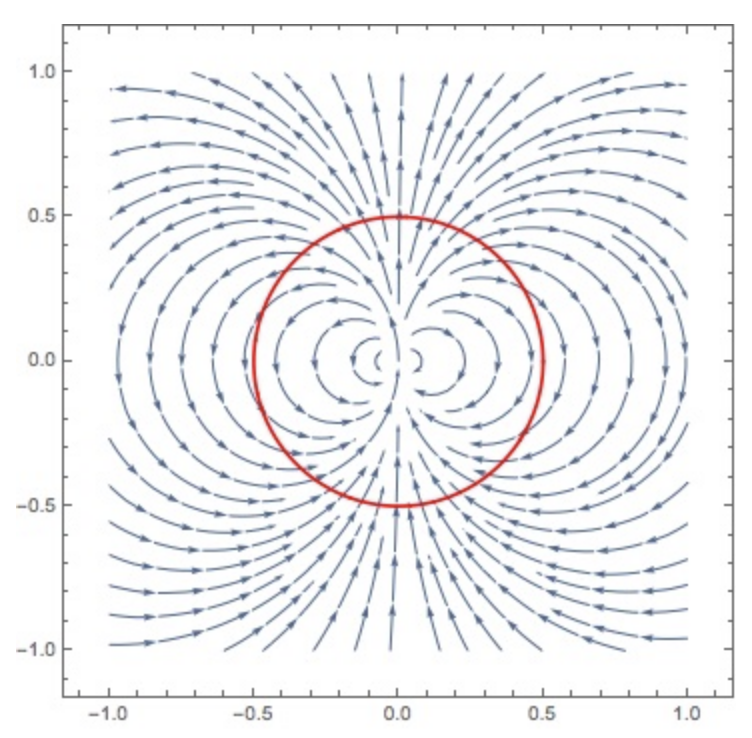
\includegraphics[width=3in]{img/C13indexcheckyourself.png}
\end{enumerate}

\vspace{0.2cm}
\hrule
\vspace{0.2cm}


\noindent\textbf{Skill Check C14 practice}
\begin{questions}
\item Retake of skill check C11 on plotting nullclines and representative vectors.

\item According to index theory, is the following phase diagram configuration possible or not?  Briefly support your answer.

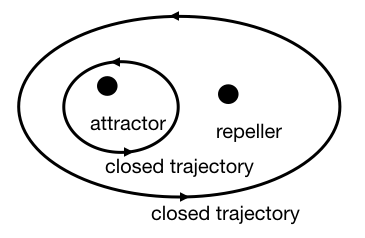
\includegraphics[]{img/C15-2019-10-07p2.png}

\noindent\textbf{Check one:}
\begin{tabular}{c |p{1cm}|}
\cline{2-2}
yes (it is possible): & \\
\cline{2-2}
no (it is not possible): & \\
\cline{2-2}
\end{tabular}

\vspace{0.2cm}

\hrule
\vspace{0.2cm}
\end{questions}



\noindent\textbf{Skill check C14 practice solution}

Each closed trajectory has an index of $+1$, so needs to enclose fixed points with a total index of $+1$, but the outer one encloses fixed points with a total index of $+2$, so not possible.


\vspace{0.2cm}
\hrule
\vspace{0.2cm}





\eject



\vspace{0.2cm}

\hrule
\vspace{0.2cm}


\begin{questions}
\item 
\begin{parts}
\item Sketch a phase portrait for a system with a saddle point at the origin.
\item Choose a closed curve that encloses the saddle point.  Find the index on that curve.
\item Choose a different closed curve and convince yourself the index is the same.
\item When a closed curve is a trajectory of the system it has an index of $+1$.   According to index theory, if the fixed point at the origin is the sole fixed point in the system, can a closed trajectory exist?
\item Now add a stable spiral at $(1,0)$.  No need to connect the two local pictures up.
\item Calculate the index about a curve that encircles just the stable spiral.
\item Could a closed trajectory exist in this new system?  If so, where? 
\end{parts}


\question (Closed orbits) Let \begin{align*}
\dot{x} &= y \\
\dot{y} &= x-x^3 - \delta y + x^2y, \quad \delta \geq 0.
\end{align*}
This can also be written $\ddot{x} = x- x^3 - \delta \dot{x} + x^2 \dot{x}$. 

This is a variation on the unforced Duffing oscillator (Duffing published work on this kind of equation in 1918, and it became a popular model in the 1970s).  \emph{Example taken from Wiggins 2003}.

Use index theory to put limits on where closed trajectories might exist.
\begin{itemize}
\item Identify the fixed points.
\item Use the determinant of the Jacobian matrix to determine the associated index for each fixed point.
\item Sketch all of the possible configurations of closed trajectories in the system, based on the index information.
\end{itemize}
\end{questions}

\eject

1a: A saddle point has two unstable directions that alternate with two stable directions.  Number these 1-4.  Let (1) point in (stable).  Then (2) points out, (3) points in, and (4) points out.  You can add additional vectors in between if you like.

1b: Align a pen with (1) so that the cap points in.  Then rotate the pen to align with (2).  The pen rotation $-90$ degrees.  To go from (2) to (3) it rotates another $-90$.  In total it will rotate $-360$ so the index is $-1$.

1c: We used the existence of the stable and unstable manifolds to figure out the index, so the curve shouldn't matter.  Any curve enclosing just a saddle point will need to cross those manifolds (the manifolds can't cross each other).  But maybe there is a way to make the manifolds swirl around or something so that there is a curve they don't cross.  That wouldn't work because trajectories point opposite directions along the manifolds so they can't get too close to each other... 

1d: No.  The saddle has an index of $-1$ so it can't be surrounded by a closed trajectory.

1e: 

1f: This index should be $+1$.

1g: Yes, it would have to be around just the stable spiral.

2a: fixed points have $y = 0$ so $x-x^3 = 0 \Rightarrow x(1-x^2) = 0$. Fixed points are $(0,0)$, $(1,0)$, $(-1,0)$.

2b: Jacobian is $\left(\begin{array}{c c}0 & 1 \\ 1-3x^2+2xy & -\delta + x^2\end{array}\right)$.  Determinant is $-1+3x^2-2xy$.  For $(0,0)$ this is $-1$ (saddle point).  For $(1,0)$ this is $-1+3 = 2$ and for $(-1,0)$ this is $-1+3=2$.  The index of the origin is $-1$ while the index of the other two fixed points is $+1$.

2c: There are three possibilities: around either of the index $+1$ fixed points, or surrounding all three fixed points.
\end{document}